\chapter{Introduction} \label{chapter1}

\tab This is a very short guide to an unofficial thesis/dissertation template
for the University of Tennessee.
It is based on the 2017 thesis specifications but can be easily altered
as the guidelines are changed.
This template requires a basic knowledge of \LaTeX\ and should cover
the basic requirements in terms of required packages and functionality.
for the University of Tennessee.

\begin{figure}[!b]
  \centering
  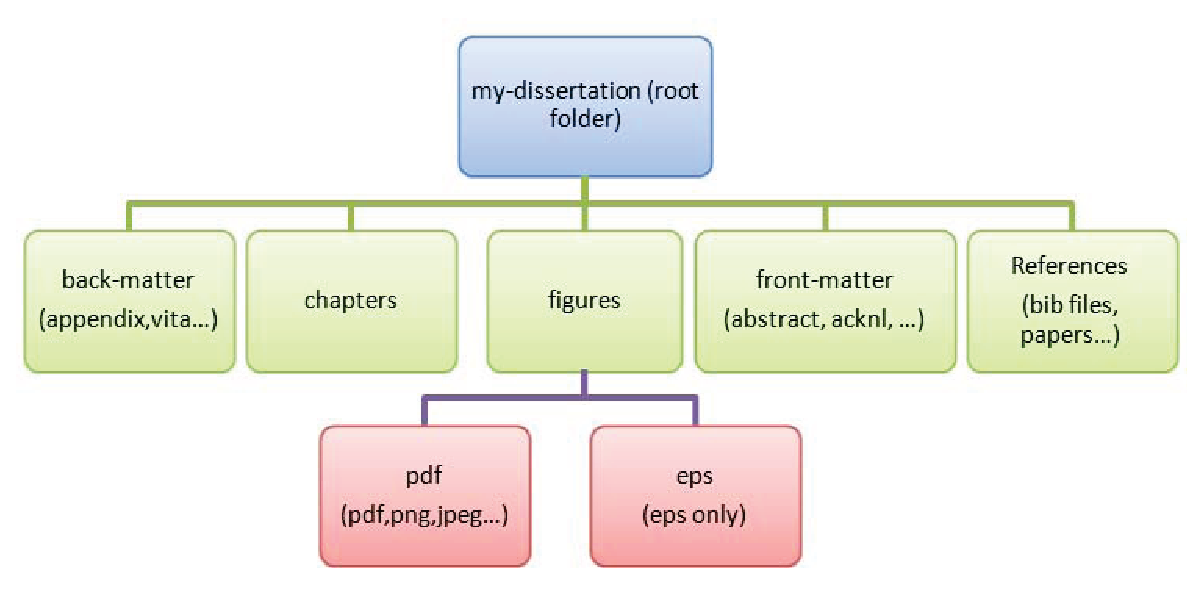
\includegraphics[width=6in]{fig01-folder-structure}
  \caption{UT thesis template folder structure.}
  \label{intro-folder-structure}
\end{figure}

\tab The general structure of this template is based on the tree shown in
\autoref{intro-folder-structure}.
The titles of the folders are self descriptive and should guide you to proper file placement.
Note that this is only a suggested model that could be
modified to fit your own organizational structure.

\section{A Section} \label{asection}
This is a paragraph found in a section part.

\subsection{A subsection}
This is a paragraph found in a subsection part.
For more information, check: \url{http://en.wikibooks.org/wiki/LaTeX/Floats,_Figures_and_Captions}

\subsubsection{A subsubsection}
This is a paragraph found in a subsubsection part.

\section{Multipart figures}
This is a paragraph found in another section part.
For multipart figures, you need to use the package ``subfig''. here's an example
\begin{figure}[!htb]
        \centering
        \subfloat[Circle]{
            \label{figure-a}
            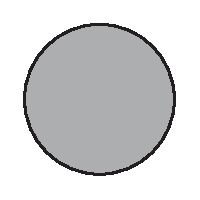
\includegraphics[width=1.1in]{fig02a-circle}
        }
        \subfloat[Rectangle]{
            \label{figure-b}
            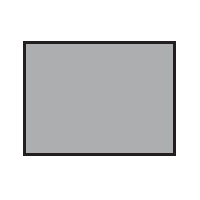
\includegraphics[width=1.1in]{fig02b-rectangle}
        }
        \subfloat[Cube]{
            \label{figure-c}
            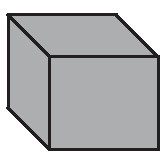
\includegraphics[width=1.1in]{fig02c-cube}
        }
        \caption{Geometric shapes.}
        \label{multipart-figure}
\end{figure}

\begin{table}[!htb]
    \centering
    \begin{tabular}{|c|c|c|c|}
        \hline
        col1 & col2 & col3 \\
        \hline
        \multirow{3}{4em}{Multiple row} & cell2 & cell3 \\
        & cell5 & cell6 \\
        & cell8 & cell9 \\
        \hline
    \end{tabular}
    \caption{An table example.}
    \label{multirow-table}
\end{table}

Discussing some analysis results from \autoref{multirow-table}.
It all started at \autoref{asection} and never ended~\dots.

